% Generated 2020-06-24 14:26:18 -0700
\subsection{Data Items} \label{model:DataItems}

\begin{figure}[ht]
  \centering
    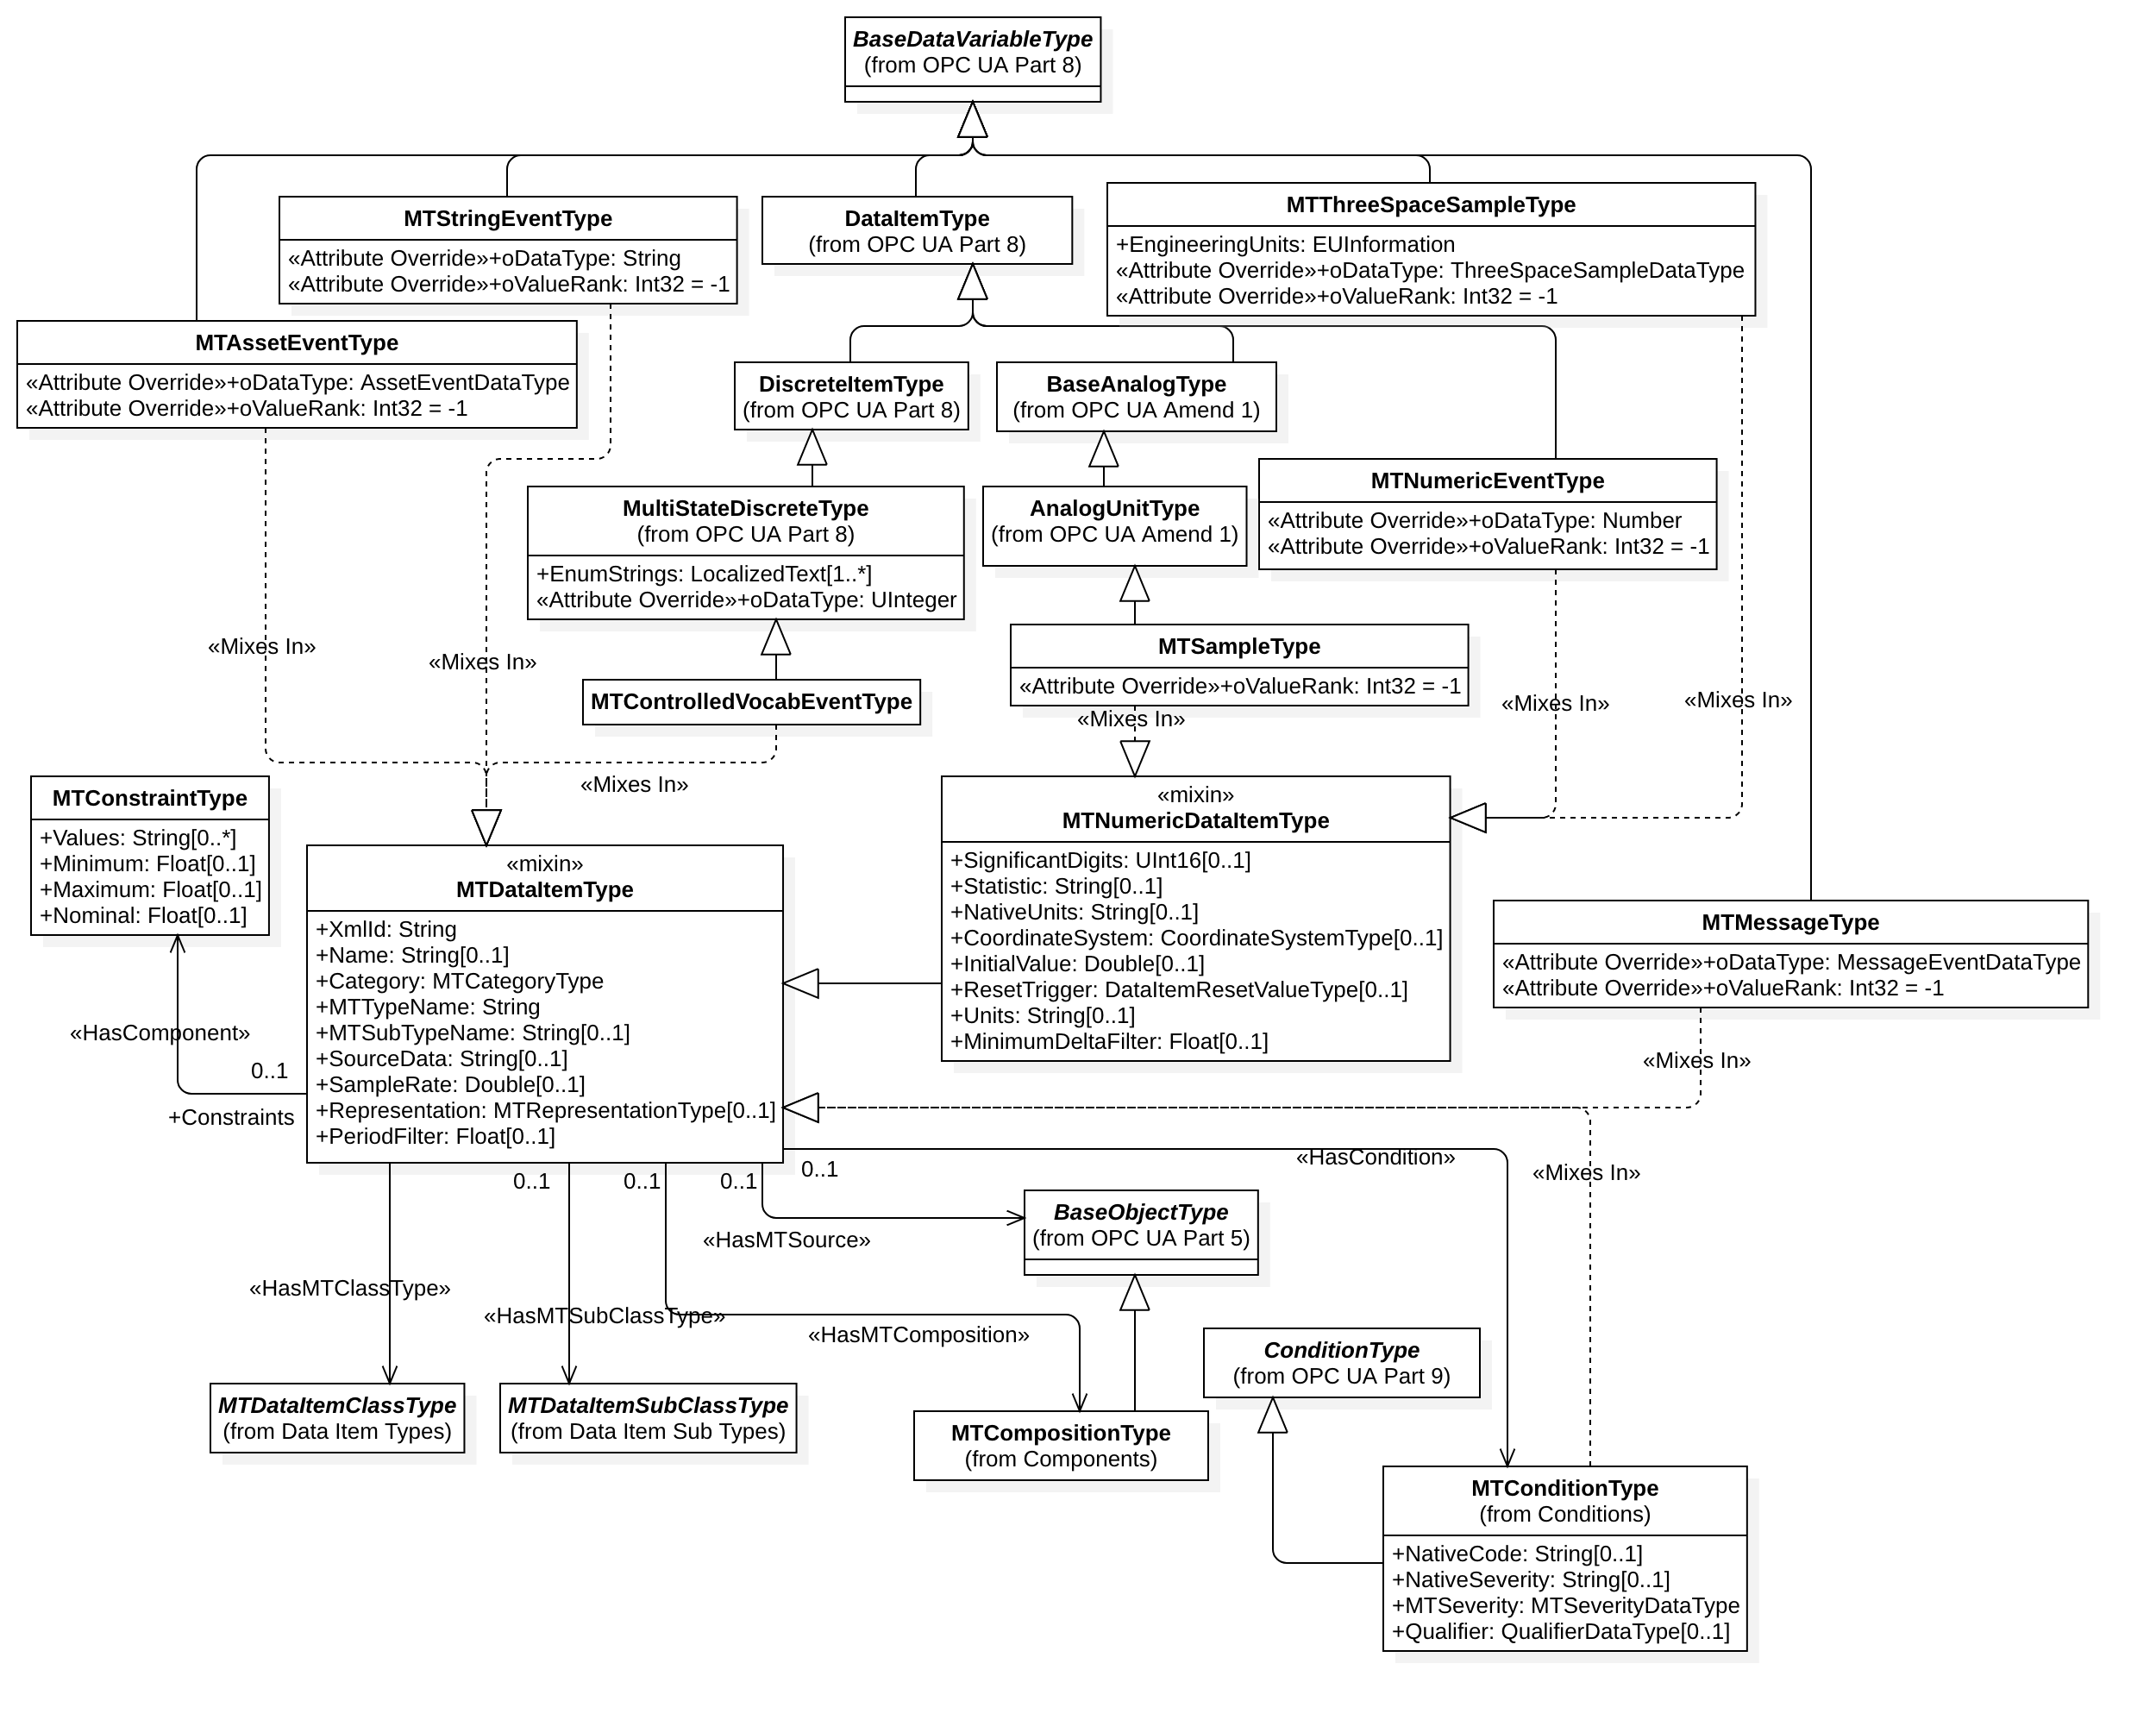
\includegraphics[width=1.0\textwidth]{./diagrams/types/DataItems.png}
  \caption{Data Items Diagram}
  \label{fig:DataItems}
\end{figure}

\FloatBarrier


\input ./type-sections/DataItems.tex

\subsubsection{Defintion of \texttt{ AssetEventDataType}}
  \label{type:AssetEventDataType}

\FloatBarrier

A special \gls{Variable} data type for asset change with a \mtmodel{AssetType} and \mtmodel{AssetId}.

\begin{table}[ht]
\centering 
  \caption{\texttt{AssetEventDataType} DataType}
  \label{data-type:AssetEventDataType}
\tabulinesep=3pt
\begin{tabu} to 6in {|l|l|l|} \everyrow{\hline}
\hline
\rowfont\bfseries {Field} & {Type} & {Optional} \\
\tabucline[1.5pt]{}
\texttt{AssetId} & \texttt{String} & \texttt{Mandatory} \\
\texttt{AssetType} & \texttt{String} & \texttt{Mandatory} \\
\end{tabu}
\end{table} 

\FloatBarrier
\paragraph{Data Type Fields}

\begin{itemize}
\item \texttt{AssetId : String:}  The unique identifier for the mtconnect asset. The identifier MUST be unique with respect to all other asset in an MTConnect installation. The identifier SHOULD be globally unique with respect to all other asset.

\item \texttt{AssetType : String:}  The type of asset that was updated.

\end{itemize}
\FloatBarrier
\subsubsection{Defintion of \texttt{ MTAssetEventType}}
  \label{type:MTAssetEventType}

\FloatBarrier

The asset events have an additional attribute regarding the asset change or removal identifier
and the type of asset that is being reported.

\begin{table}[ht]
\centering 
  \caption{\texttt{MTAssetEventType} Definition}
  \label{table:MTAssetEventType}
\fontsize{9pt}{11pt}\selectfont
\tabulinesep=3pt
\begin{tabu} to 6in {|X[-1.35]|X[-0.7]|X[-1.75]|X[-1.5]|X[-1]|X[-0.7]|} \everyrow{\hline}
\hline
\rowfont\bfseries {Attribute} & \multicolumn{5}{|l|}{Value} \\
\tabucline[1.5pt]{}
BrowseName & \multicolumn{5}{|l|}{MTAssetEventType} \\
IsAbstract & \multicolumn{5}{|l|}{False} \\
ValueRank & \multicolumn{5}{|l|}{-1} \\
DataType & \multicolumn{5}{|l|}{AssetEventDataType} \\
\tabucline[1.5pt]{}
\rowfont \bfseries References & NodeClass & BrowseName & DataType & Type\-Definition & {Modeling\-Rule} \\
\multicolumn{6}{|l|}{Subtype of BaseDataVariableType (See \cite{UAPart8} Documentation)} \\
Has\-Property & Variable & Category & MT\-Category\-Type & Property\-Type & Mandatory \\
Has\-Property & Variable & MT\-Sub\-Type\-Name & String & Property\-Type & Optional \\
Has\-Property & Variable & MT\-Type\-Name & String & Property\-Type & Mandatory \\
Has\-Property & Variable & Name & String & Property\-Type & Optional \\
Has\-Property & Variable & Period\-Filter & Float & Property\-Type & Optional \\
Has\-Property & Variable & Representation & MT\-Representation\-Type & Property\-Type & Optional \\
Has\-Property & Variable & Sample\-Rate & Double & Property\-Type & Optional \\
Has\-Property & Variable & Source\-Data & String & Property\-Type & Optional \\
Has\-Property & Variable & Xml\-Id & String & Property\-Type & Mandatory \\
Has\-MT\-Source & Object & <Base\-Object> & \multicolumn{2}{l|}{BaseObjectType} & Optional \\
Has\-MT\-Composition & Object & <MT\-Composition> & \multicolumn{2}{l|}{MTCompositionType} & Optional \\
Has\-MT\-Sub\-Class\-Type & Object & <MT\-Data\-Item\-Sub\-Class> & \multicolumn{2}{l|}{MTDataItemSubClassType} & Optional \\
Has\-Condition & Object & <MT\-Condition> & \multicolumn{2}{l|}{MTConditionType} & Optional \\
Has\-Component & Object & Constraints & \multicolumn{2}{l|}{MTConstraintType} & Optional \\
Has\-MT\-Class\-Type & Object & <MT\-Data\-Item\-Class> & \multicolumn{2}{l|}{MTDataItemClassType} & Mandatory \\
\end{tabu}
\end{table} 


\paragraph{Dependencies and Relationships}

\begin{itemize}
\item Mixes in \texttt{MTDataItemType}, see See section \ref{type:MTDataItemType}
\end{itemize}
\FloatBarrier
\subsubsection{Defintion of \texttt{ MTConditionClassType}}
  \label{type:MTConditionClassType}

\FloatBarrier

The abstract type for all data items types that are specifically for \mtmodel{CONDITION} \gls{category}.

An XML element which provides the information and data reported from a piece of equipment for those dataitem elements defined with a category attribute of condition category in the mtconnectdevices document.

\begin{table}[ht]
\centering 
  \caption{\texttt{MTConditionClassType} Definition}
  \label{table:MTConditionClassType}
\fontsize{9pt}{11pt}\selectfont
\tabulinesep=3pt
\begin{tabu} to 6in {|X[-1.35]|X[-0.7]|X[-1.75]|X[-1.5]|X[-1]|X[-0.7]|} \everyrow{\hline}
\hline
\rowfont\bfseries {Attribute} & \multicolumn{5}{|l|}{Value} \\
\tabucline[1.5pt]{}
BrowseName & \multicolumn{5}{|l|}{MTConditionClassType} \\
IsAbstract & \multicolumn{5}{|l|}{True} \\
\tabucline[1.5pt]{}
\rowfont \bfseries References & NodeClass & BrowseName & DataType & Type\-Definition & {Modeling\-Rule} \\
\multicolumn{6}{|l|}{Subtype of MTDataItemClassType (See Data Item Types Documentation)} \\
HasSubtype & ObjectType & \multicolumn{2}{l}{ActuatorClassType} & \multicolumn{2}{|l|}{See section \ref{type:ActuatorClassType}} \\
HasSubtype & ObjectType & \multicolumn{2}{l}{CommunicationsClassType} & \multicolumn{2}{|l|}{See section \ref{type:CommunicationsClassType}} \\
HasSubtype & ObjectType & \multicolumn{2}{l}{DataRangeClassType} & \multicolumn{2}{|l|}{See section \ref{type:DataRangeClassType}} \\
HasSubtype & ObjectType & \multicolumn{2}{l}{HardwareClassType} & \multicolumn{2}{|l|}{See section \ref{type:HardwareClassType}} \\
HasSubtype & ObjectType & \multicolumn{2}{l}{LogicProgramClassType} & \multicolumn{2}{|l|}{See section \ref{type:LogicProgramClassType}} \\
HasSubtype & ObjectType & \multicolumn{2}{l}{MotionProgramClassType} & \multicolumn{2}{|l|}{See section \ref{type:MotionProgramClassType}} \\
HasSubtype & ObjectType & \multicolumn{2}{l}{SystemClassType} & \multicolumn{2}{|l|}{See section \ref{type:SystemClassType}} \\
\end{tabu}
\end{table} 


\FloatBarrier
\subsubsection{Defintion of \texttt{ MTConstraintType}}
  \label{type:MTConstraintType}

\FloatBarrier

The MTConnect constraints. The Values or the Minimum, Maximum, and Nominal values should be 
provided. Multiple Values can be provided as an array as a set of allowable values for this
\gls{MTDataItem}.

A constraint is used by a software application to evaluate the validity of the reported data.

\begin{table}[ht]
\centering 
  \caption{\texttt{MTConstraintType} Definition}
  \label{table:MTConstraintType}
\fontsize{9pt}{11pt}\selectfont
\tabulinesep=3pt
\begin{tabu} to 6in {|X[-1.35]|X[-0.7]|X[-1.75]|X[-1.5]|X[-1]|X[-0.7]|} \everyrow{\hline}
\hline
\rowfont\bfseries {Attribute} & \multicolumn{5}{|l|}{Value} \\
\tabucline[1.5pt]{}
BrowseName & \multicolumn{5}{|l|}{MTConstraintType} \\
IsAbstract & \multicolumn{5}{|l|}{False} \\
\tabucline[1.5pt]{}
\rowfont \bfseries References & NodeClass & BrowseName & DataType & Type\-Definition & {Modeling\-Rule} \\
\multicolumn{6}{|l|}{Subtype of BaseObjectType (See \cite{UAPart5} Documentation)} \\
Has\-Property & Variable & Maximum & Float & Property\-Type & Optional \\
Has\-Property & Variable & Minimum & Float & Property\-Type & Optional \\
Has\-Property & Variable & Nominal & Float & Property\-Type & Optional \\
Has\-Property & Variable & Values & String[] & Property\-Type & Optional \\
\end{tabu}
\end{table} 


\FloatBarrier
\paragraph{Referenced Properties and Objects}

\begin{itemize}
\item \texttt{Maximum : Float:}  The upper limit of data reported for a data item.

\item \texttt{Minimum : Float:}  The lower limit of data reported for a data item.

\item \texttt{Nominal : Float:}  The target or expected value for this data item.

\end{itemize}
\FloatBarrier
\subsubsection{Defintion of \texttt{ MTControlledVocabEventType}}
  \label{type:MTControlledVocabEventType}

\FloatBarrier

All \glspl{MTDataItem} with \gls{category} \mtmodel{EVENT} having Controlled Vocabularies (Enumerations) 
will be added as sub-types of this type which is mapped to the OPC/UA MultiStateValueDiscreteType. 
Otherwise, either \mtmodel{MTString} or \mtmodel{MTNumeric} will be used. All subtypes are direct representations of the 
MTConnect equivalent elements that can be found in the MTConnect Part 3 \cite{MTCPart3} documents.

\begin{table}[ht]
\centering 
  \caption{\texttt{MTControlledVocabEventType} Definition}
  \label{table:MTControlledVocabEventType}
\fontsize{9pt}{11pt}\selectfont
\tabulinesep=3pt
\begin{tabu} to 6in {|X[-1.35]|X[-0.7]|X[-1.75]|X[-1.5]|X[-1]|X[-0.7]|} \everyrow{\hline}
\hline
\rowfont\bfseries {Attribute} & \multicolumn{5}{|l|}{Value} \\
\tabucline[1.5pt]{}
BrowseName & \multicolumn{5}{|l|}{MTControlledVocabEventType} \\
IsAbstract & \multicolumn{5}{|l|}{False} \\
ValueRank & \multicolumn{5}{|l|}{-1} \\
DataType & \multicolumn{5}{|l|}{UInteger} \\
\tabucline[1.5pt]{}
\rowfont \bfseries References & NodeClass & BrowseName & DataType & Type\-Definition & {Modeling\-Rule} \\
\multicolumn{6}{|l|}{Subtype of MultiStateDiscreteType (See \cite{UAPart8} Documentation)} \\
Has\-Property & Variable & Category & MT\-Category\-Type & Property\-Type & Mandatory \\
Has\-Property & Variable & MT\-Sub\-Type\-Name & String & Property\-Type & Optional \\
Has\-Property & Variable & MT\-Type\-Name & String & Property\-Type & Mandatory \\
Has\-Property & Variable & Name & String & Property\-Type & Optional \\
Has\-Property & Variable & Period\-Filter & Float & Property\-Type & Optional \\
Has\-Property & Variable & Representation & MT\-Representation\-Type & Property\-Type & Optional \\
Has\-Property & Variable & Sample\-Rate & Double & Property\-Type & Optional \\
Has\-Property & Variable & Source\-Data & String & Property\-Type & Optional \\
Has\-Property & Variable & Xml\-Id & String & Property\-Type & Mandatory \\
Has\-MT\-Source & Object & <Base\-Object> & \multicolumn{2}{l|}{BaseObjectType} & Optional \\
Has\-MT\-Composition & Object & <MT\-Composition> & \multicolumn{2}{l|}{MTCompositionType} & Optional \\
Has\-MT\-Sub\-Class\-Type & Object & <MT\-Data\-Item\-Sub\-Class> & \multicolumn{2}{l|}{MTDataItemSubClassType} & Optional \\
Has\-Condition & Object & <MT\-Condition> & \multicolumn{2}{l|}{MTConditionType} & Optional \\
Has\-Component & Object & Constraints & \multicolumn{2}{l|}{MTConstraintType} & Optional \\
Has\-MT\-Class\-Type & Object & <MT\-Data\-Item\-Class> & \multicolumn{2}{l|}{MTDataItemClassType} & Mandatory \\
Has\-Property & Variable & Value\-As\-Text & String & Property\-Type & Mandatory \\
\end{tabu}
\end{table} 


\paragraph{Dependencies and Relationships}

\begin{itemize}
\item Mixes in \texttt{MTDataItemType}, see See section \ref{type:MTDataItemType}
\end{itemize}
\FloatBarrier
\subsubsection{Defintion of \texttt{<<mixin>> MTDataItemType}}
  \label{type:MTDataItemType}

\FloatBarrier

The data item mixin will inject the properties and the methods into the related 
classes. This facility is similar to the Ruby module mixin or the Scala traits.

data entity describing a piece of information reported about a piece of equipment.

\begin{table}[ht]
\centering 
  \caption{\texttt{MTDataItemType} Definition}
  \label{table:MTDataItemType}
\fontsize{9pt}{11pt}\selectfont
\tabulinesep=3pt
\begin{tabu} to 6in {|X[-1.35]|X[-0.7]|X[-1.75]|X[-1.5]|X[-1]|X[-0.7]|} \everyrow{\hline}
\hline
\rowfont\bfseries {Attribute} & \multicolumn{5}{|l|}{Value} \\
\tabucline[1.5pt]{}
BrowseName & \multicolumn{5}{|l|}{MTDataItemType} \\
IsAbstract & \multicolumn{5}{|l|}{False} \\
\tabucline[1.5pt]{}
\rowfont \bfseries References & NodeClass & BrowseName & DataType & Type\-Definition & {Modeling\-Rule} \\
HasSubtype & ObjectType & \multicolumn{2}{l}{MTNumericDataItemType} & \multicolumn{2}{|l|}{See section \ref{type:MTNumericDataItemType}} \\
Has\-Property & Variable & Category & MT\-Category\-Type & Property\-Type & Mandatory \\
Has\-Property & Variable & MT\-Sub\-Type\-Name & String & Property\-Type & Optional \\
Has\-Property & Variable & MT\-Type\-Name & String & Property\-Type & Mandatory \\
Has\-Property & Variable & Name & String & Property\-Type & Optional \\
Has\-Property & Variable & Period\-Filter & Float & Property\-Type & Optional \\
Has\-Property & Variable & Representation & MT\-Representation\-Type & Property\-Type & Optional \\
Has\-Property & Variable & Sample\-Rate & Double & Property\-Type & Optional \\
Has\-Property & Variable & Source\-Data & String & Property\-Type & Optional \\
Has\-Property & Variable & Xml\-Id & String & Property\-Type & Mandatory \\
Has\-MT\-Source & Object & <Base\-Object> & \multicolumn{2}{l|}{BaseObjectType} & Optional \\
Has\-MT\-Composition & Object & <MT\-Composition> & \multicolumn{2}{l|}{MTCompositionType} & Optional \\
Has\-MT\-Sub\-Class\-Type & Object & <MT\-Data\-Item\-Sub\-Class> & \multicolumn{2}{l|}{MTDataItemSubClassType} & Optional \\
Has\-Condition & Object & <MT\-Condition> & \multicolumn{2}{l|}{MTConditionType} & Optional \\
Has\-Component & Object & Constraints & \multicolumn{2}{l|}{MTConstraintType} & Optional \\
Has\-MT\-Class\-Type & Object & <MT\-Data\-Item\-Class> & \multicolumn{2}{l|}{MTDataItemClassType} & Mandatory \\
\end{tabu}
\end{table} 


\FloatBarrier
\paragraph{Referenced Properties and Objects}

\begin{itemize}
\item \texttt{Category : MTCategoryType:}  Specifies the kind of information provided by a data item. 

\item \textbf{Allowable Values} for \texttt{MTCategoryType}
\FloatBarrier

Represents the \gls{category} attribute of the MTConnect \gls{MTDataItem}.

\begin{table}[ht]
\centering 
  \caption{\texttt{MTCategoryType} Enumeration}
  \label{enum:MTCategoryType}
\tabulinesep=3pt
\begin{tabu} to 6in {|l|r|X|} \everyrow{\hline}
\hline
\rowfont\bfseries {Name} & {Index} & {Description} \\
\tabucline[1.5pt]{}
\texttt{EVENT} & \texttt{0} & An event category is a data item representing a discrete piece of information from the piece of equipment.  \\
\texttt{CONDITION} & \texttt{1} & A condition category is a data item that communicates information about the health of a piece of equipment and its ability to function.  \\
\texttt{SAMPLE} & \texttt{2} & A sample category is the reading of the value of a continuously variable or analog data value. \\
\end{tabu}
\end{table} 
\FloatBarrier
\item \texttt{Name : String:}  The name of an element or a piece of equipment.

\item \texttt{PeriodFilter : Float:} Represents the MTConnect \mtmodel{Filter} subtype of \mtmodel{PeriodFilter}.

\item \texttt{Representation : MTRepresentationType:}  Description of a means to interpret data consisting of multiple data points or samples reported as a single value.  
 representation is an optional attribute.  
 representation will define a unique format for each set of data.  
 representation for timeseries representation, discrete representation, and value representation are defined in MTCPart2 Section 7.2.2.12.  
 If representation is not specified, it MUST be determined to be value representation.

\item \textbf{Allowable Values} for \texttt{MTRepresentationType}
\FloatBarrier

Represents the \mtmodel{representation} attribute of the MTConnect \gls{MTDataItem}.

\begin{table}[ht]
\centering 
  \caption{\texttt{MTRepresentationType} Enumeration}
  \label{enum:MTRepresentationType}
\tabulinesep=3pt
\begin{tabu} to 6in {|l|r|X|} \everyrow{\hline}
\hline
\rowfont\bfseries {Name} & {Index} & {Description} \\
\tabucline[1.5pt]{}
\texttt{DISCRETE} & \texttt{0} & A data entity where each discrete occurrence of the data may have the same value as the previous occurrence of the data. \\
\texttt{TIME_SERIES} & \texttt{1} & A series of sampled data.  \\
\texttt{VALUE} & \texttt{2} & The measured value of the sample data. \\
\end{tabu}
\end{table} 
\FloatBarrier
\item \texttt{SampleRate : Double:}  The rate at which successive samples of a data item are recorded by a piece of equipment.

\item \texttt{SourceData : String:} The text that is the \gls{CDATA} of the \mtmodel{Source} element.

\end{itemize}
\FloatBarrier
\subsubsection{Defintion of \texttt{<<mixin>> MTNumericDataItemType}}
  \label{type:MTNumericDataItemType}

\FloatBarrier

These are the additional attributes that are relevent to numeric data items. 
The factory will evaluate these values and will set the engineering units and the 
range associated with the parent entity.

\begin{table}[ht]
\centering 
  \caption{\texttt{MTNumericDataItemType} Definition}
  \label{table:MTNumericDataItemType}
\fontsize{9pt}{11pt}\selectfont
\tabulinesep=3pt
\begin{tabu} to 6in {|X[-1.35]|X[-0.7]|X[-1.75]|X[-1.5]|X[-1]|X[-0.7]|} \everyrow{\hline}
\hline
\rowfont\bfseries {Attribute} & \multicolumn{5}{|l|}{Value} \\
\tabucline[1.5pt]{}
BrowseName & \multicolumn{5}{|l|}{MTNumericDataItemType} \\
IsAbstract & \multicolumn{5}{|l|}{False} \\
\tabucline[1.5pt]{}
\rowfont \bfseries References & NodeClass & BrowseName & DataType & Type\-Definition & {Modeling\-Rule} \\
\multicolumn{6}{|l|}{Subtype of MTDataItemType (See section \ref{type:MTDataItemType})} \\
Has\-Property & Variable & Coordinate\-System & MT\-Coordinate\-System\-Type & Property\-Type & Optional \\
Has\-Property & Variable & Duration & Duration & Property\-Type & Optional \\
Has\-Property & Variable & Initial\-Value & Double & Property\-Type & Optional \\
Has\-Property & Variable & Minimum\-Delta\-Filter & Float & Property\-Type & Optional \\
Has\-Property & Variable & Native\-Units & String & Property\-Type & Optional \\
Has\-Property & Variable & Reset\-Trigger & MT\-Reset\-Trigger\-Type & Property\-Type & Optional \\
Has\-Property & Variable & Reset\-Triggered\-Reason & MT\-Reset\-Trigger\-Type & Property\-Type & Optional \\
Has\-Property & Variable & Significant\-Digits & Int16 & Property\-Type & Optional \\
Has\-Property & Variable & Statistic & MT\-Statistic\-Type & Property\-Type & Optional \\
Has\-Property & Variable & Units & String & Property\-Type & Optional \\
\end{tabu}
\end{table} 


\FloatBarrier
\paragraph{Referenced Properties and Objects}

\begin{itemize}
\item \texttt{CoordinateSystem : MTCoordinateSystemType:}  For measured values relative to a coordinate system like position sample, the coordinate system being used may be reported.

\item \textbf{Allowable Values} for \texttt{MTCoordinateSystemType}
\FloatBarrier

Represents the \mtmodel{coordinateSystem} attribute of the MTConnect \gls{MTDataItem}.

It is a reference system that associates a unique set of n parameters with each point in an n-dimensional space. Ref: ISO 10303-218:2004

\begin{table}[ht]
\centering 
  \caption{\texttt{MTCoordinateSystemType} Enumeration}
  \label{enum:MTCoordinateSystemType}
\tabulinesep=3pt
\begin{tabu} to 6in {|l|r|X|} \everyrow{\hline}
\hline
\rowfont\bfseries {Name} & {Index} & {Description} \\
\tabucline[1.5pt]{}
\texttt{MACHINE} & \texttt{0} & An unchangeable coordinate system that has machine zero as its origin. \\
\texttt{WORK} & \texttt{1} & The coordinate system that represents the working area for a particular workpiece whose origin is shifted within the machine coordinate system. If the work coordinates are not currently defined in the piece of equipment, the machine coordinates will be used. \\
\end{tabu}
\end{table} 
\FloatBarrier
\item \texttt{Duration : Duration:}  The time-period over which the data was collected.

\item \texttt{InitialValue : Double:}  initialvalue is an optional XML element that defines the starting value for a data item as well as the value to be set for the data item after a reset event.

\item \texttt{MinimumDeltaFilter : Float:} Represents the MTConnect \mtmodel{Filter} subtype of \mtmodel{MinimumDeltaFilter}.

\item \texttt{NativeUnits : String:}  The native units of measurement for the reported value of the data item.

\item \texttt{ResetTrigger : MTResetTriggerType:} If a \mtmodel{ResetTrigger} is given, when an \mtmodel{resetTriggered} attribtue is given in an event, the \uamodel{StatusCode} MUST have bit 14 set \uamodel{SemanticsChanged} and the \mtmodel{ResetTriggeredReason} must be set to the value of the \mtmodel{resetTriggered} attribute. resettrigger is an optional XML element that identifies the type of event that may cause a reset to occur. It is additional information regarding the meaning of the data that establishes an understanding of the time frame that the data represents so that the data may be correctly understood by a client software application.

\item \textbf{Allowable Values} for \texttt{MTResetTriggerType}
\FloatBarrier

These need to become \uamodel{Good_} status code in OPC UA.

resettrigger is an optional XML element that identifies the type of event that may cause a reset to occur. It is additional information regarding the meaning of the data that establishes an understanding of the time frame that the data represents so that the data may be correctly understood by a client software application.

\begin{table}[ht]
\centering 
  \caption{\texttt{MTResetTriggerType} Enumeration}
  \label{enum:MTResetTriggerType}
\tabulinesep=3pt
\begin{tabu} to 6in {|l|r|X|} \everyrow{\hline}
\hline
\rowfont\bfseries {Name} & {Index} & {Description} \\
\tabucline[1.5pt]{}
\texttt{ACTION_COMPLETE} & \texttt{0} & The value of the data entity that is measuring an action or operation is to be reset upon completion of that action or operation. \\
\texttt{ANNUAL} & \texttt{1} & The value of the data entity is to be reset at the end of a 12-month period. \\
\texttt{DAY} & \texttt{2} & The value of the data entity is to be reset at the end of a 24-hour period. \\
\texttt{MAINTENANCE} & \texttt{3} & Action related to maintenance on the piece of equipment. \\
\texttt{MANUAL} & \texttt{4} & Operations based on the instructions received from an external source. \\
\texttt{MONTH} & \texttt{5} & The value of the data entity is to be reset at the end of a monthly period. \\
\texttt{POWER_ON} & \texttt{6} & The value of the data entity is to be reset when power was applied to the piece of equipment after a planned or unplanned interruption of power has occurred. \\
\texttt{SHIFT} & \texttt{7} & The value of the data entity is to be reset at the end of a work shift. \\
\texttt{WEEK} & \texttt{8} & The value of the data entity is to be reset at the end of a 7-day period. \\
\end{tabu}
\end{table} 
\FloatBarrier
\item \textbf{Allowable Values} for \texttt{MTResetTriggerType}
\FloatBarrier

These need to become \uamodel{Good_} status code in OPC UA.

resettrigger is an optional XML element that identifies the type of event that may cause a reset to occur. It is additional information regarding the meaning of the data that establishes an understanding of the time frame that the data represents so that the data may be correctly understood by a client software application.

\begin{table}[ht]
\centering 
  \caption{\texttt{MTResetTriggerType} Enumeration}
\tabulinesep=3pt
\begin{tabu} to 6in {|l|r|X|} \everyrow{\hline}
\hline
\rowfont\bfseries {Name} & {Index} & {Description} \\
\tabucline[1.5pt]{}
\texttt{ACTION_COMPLETE} & \texttt{0} & The value of the data entity that is measuring an action or operation is to be reset upon completion of that action or operation. \\
\texttt{ANNUAL} & \texttt{1} & The value of the data entity is to be reset at the end of a 12-month period. \\
\texttt{DAY} & \texttt{2} & The value of the data entity is to be reset at the end of a 24-hour period. \\
\texttt{MAINTENANCE} & \texttt{3} & Action related to maintenance on the piece of equipment. \\
\texttt{MANUAL} & \texttt{4} & Operations based on the instructions received from an external source. \\
\texttt{MONTH} & \texttt{5} & The value of the data entity is to be reset at the end of a monthly period. \\
\texttt{POWER_ON} & \texttt{6} & The value of the data entity is to be reset when power was applied to the piece of equipment after a planned or unplanned interruption of power has occurred. \\
\texttt{SHIFT} & \texttt{7} & The value of the data entity is to be reset at the end of a work shift. \\
\texttt{WEEK} & \texttt{8} & The value of the data entity is to be reset at the end of a 7-day period. \\
\end{tabu}
\end{table} 
\FloatBarrier
\item \texttt{SignificantDigits : Int16:} The significant digits is converted to a \uaterm{ValuePrecision}. The number of significant digits in the reported value.

\item \texttt{Statistic : MTStatisticType:}  Describes the type of statistical calculation performed on a series of data samples to provide the reported data value.

\item \textbf{Allowable Values} for \texttt{MTStatisticType}
\FloatBarrier



\begin{table}[ht]
\centering 
  \caption{\texttt{MTStatisticType} Enumeration}
  \label{enum:MTStatisticType}
\tabulinesep=3pt
\begin{tabu} to 6in {|l|r|X|} \everyrow{\hline}
\hline
\rowfont\bfseries {Name} & {Index} & {Description} \\
\tabucline[1.5pt]{}
\texttt{AVERAGE} & \texttt{0} & Mathematical Average value calculated for the data item during the calculation period. \\
\texttt{MAXIMUM} & \texttt{1} & The upper limit of data reported for a data item. \\
\texttt{MEDIAN} & \texttt{2} & The middle number of a series of numbers. \\
\texttt{MINIMUM} & \texttt{3} & The lower limit of data reported for a data item. \\
\texttt{MODE} & \texttt{4} & The number in a series of numbers that occurs most often. \\
\texttt{RANGE} & \texttt{5} & Difference between the maximum and minimum value of a data item during the calculation period.  Also represents Peak-to-Peak measurement in a waveform. \\
\texttt{ROOT_MEAN_SQUARE} & \texttt{6} & Mathematical Root Mean Square (RMS) value calculated for the data item during the calculation period. \\
\texttt{STANDARD_DEVIATION} & \texttt{7} & Statistical Standard Deviation value calculated for the data item during the calculation period. \\
\end{tabu}
\end{table} 
\FloatBarrier
\item \texttt{Units : String:}  The unit of measurement for the reported value of the data item.

\end{itemize}
\FloatBarrier
\subsubsection{Defintion of \texttt{ MTEventClassType}}
  \label{type:MTEventClassType}

\FloatBarrier

The base type class for all data items with a \gls{category} of \mtmodel{EVENT}.

An XML element which provides the information and data reported from a piece of equipment for those dataitem elements defined with a category attribute of event category in the mtconnectdevices document.

\begin{table}[ht]
\centering 
  \caption{\texttt{MTEventClassType} Definition}
  \label{table:MTEventClassType}
\fontsize{9pt}{11pt}\selectfont
\tabulinesep=3pt
\begin{tabu} to 6in {|X[-1.35]|X[-0.7]|X[-1.75]|X[-1.5]|X[-1]|X[-0.7]|} \everyrow{\hline}
\hline
\rowfont\bfseries {Attribute} & \multicolumn{5}{|l|}{Value} \\
\tabucline[1.5pt]{}
BrowseName & \multicolumn{5}{|l|}{MTEventClassType} \\
IsAbstract & \multicolumn{5}{|l|}{True} \\
\tabucline[1.5pt]{}
\rowfont \bfseries References & NodeClass & BrowseName & DataType & Type\-Definition & {Modeling\-Rule} \\
\multicolumn{6}{|l|}{Subtype of MTDataItemClassType (See Data Item Types Documentation)} \\
HasSubtype & ObjectType & \multicolumn{2}{l}{MTMessageClassType} & \multicolumn{2}{|l|}{See section \ref{type:MTMessageClassType}} \\
HasSubtype & ObjectType & \multicolumn{2}{l}{MTControlledVocabEventClassType} & \multicolumn{2}{|l|}{See section \ref{type:MTControlledVocabEventClassType}} \\
HasSubtype & ObjectType & \multicolumn{2}{l}{MTNumericEventClassType} & \multicolumn{2}{|l|}{See section \ref{type:MTNumericEventClassType}} \\
HasSubtype & ObjectType & \multicolumn{2}{l}{MTStringEventClassType} & \multicolumn{2}{|l|}{See section \ref{type:MTStringEventClassType}} \\
\end{tabu}
\end{table} 


\FloatBarrier
\subsubsection{Defintion of \texttt{ MTMessageEventType}}
  \label{type:MTMessageEventType}

\FloatBarrier



\begin{table}[ht]
\centering 
  \caption{\texttt{MTMessageEventType} Definition}
  \label{table:MTMessageEventType}
\fontsize{9pt}{11pt}\selectfont
\tabulinesep=3pt
\begin{tabu} to 6in {|X[-1.35]|X[-0.7]|X[-1.75]|X[-1.5]|X[-1]|X[-0.7]|} \everyrow{\hline}
\hline
\rowfont\bfseries {Attribute} & \multicolumn{5}{|l|}{Value} \\
\tabucline[1.5pt]{}
BrowseName & \multicolumn{5}{|l|}{MTMessageEventType} \\
IsAbstract & \multicolumn{5}{|l|}{False} \\
\tabucline[1.5pt]{}
\rowfont \bfseries References & NodeClass & BrowseName & DataType & Type\-Definition & {Modeling\-Rule} \\
\multicolumn{6}{|l|}{Subtype of BaseEventType (See \cite{UAPart5} Documentation)} \\
Has\-Property & Variable & Native\-Code & String & Property\-Type & Optional \\
\end{tabu}
\end{table} 


\FloatBarrier
\paragraph{Referenced Properties and Objects}

\begin{itemize}
\item \texttt{NativeCode : String:}  The native code (usually an alpha-numeric value) generated by the controller of a piece of equipment or the element.

\end{itemize}
\FloatBarrier
\subsubsection{Defintion of \texttt{ MTMessageType}}
  \label{type:MTMessageType}

\FloatBarrier

The message is a sub-type of the \uaterm{DataVariableType} using the \mtuatype{MessageDataType} to 
represent the values for \mtterm{NativeCode} and \mtterm{Text} of the message from the \gls{CDATA} of the 
MTConnect Streams message.

Any text string of information to be transferred from a piece of equipment to a client software application.

\begin{table}[ht]
\centering 
  \caption{\texttt{MTMessageType} Definition}
  \label{table:MTMessageType}
\fontsize{9pt}{11pt}\selectfont
\tabulinesep=3pt
\begin{tabu} to 6in {|X[-1.35]|X[-0.7]|X[-1.75]|X[-1.5]|X[-1]|X[-0.7]|} \everyrow{\hline}
\hline
\rowfont\bfseries {Attribute} & \multicolumn{5}{|l|}{Value} \\
\tabucline[1.5pt]{}
BrowseName & \multicolumn{5}{|l|}{MTMessageType} \\
IsAbstract & \multicolumn{5}{|l|}{False} \\
ValueRank & \multicolumn{5}{|l|}{-1} \\
DataType & \multicolumn{5}{|l|}{MessageDataType} \\
\tabucline[1.5pt]{}
\rowfont \bfseries References & NodeClass & BrowseName & DataType & Type\-Definition & {Modeling\-Rule} \\
\multicolumn{6}{|l|}{Subtype of BaseDataVariableType (See \cite{UAPart8} Documentation)} \\
Has\-Property & Variable & Category & MT\-Category\-Type & Property\-Type & Mandatory \\
Has\-Property & Variable & MT\-Sub\-Type\-Name & String & Property\-Type & Optional \\
Has\-Property & Variable & MT\-Type\-Name & String & Property\-Type & Mandatory \\
Has\-Property & Variable & Name & String & Property\-Type & Optional \\
Has\-Property & Variable & Period\-Filter & Float & Property\-Type & Optional \\
Has\-Property & Variable & Representation & MT\-Representation\-Type & Property\-Type & Optional \\
Has\-Property & Variable & Sample\-Rate & Double & Property\-Type & Optional \\
Has\-Property & Variable & Source\-Data & String & Property\-Type & Optional \\
Has\-Property & Variable & Xml\-Id & String & Property\-Type & Mandatory \\
Has\-MT\-Source & Object & <Base\-Object> & \multicolumn{2}{l|}{BaseObjectType} & Optional \\
Has\-MT\-Composition & Object & <MT\-Composition> & \multicolumn{2}{l|}{MTCompositionType} & Optional \\
Has\-MT\-Sub\-Class\-Type & Object & <MT\-Data\-Item\-Sub\-Class> & \multicolumn{2}{l|}{MTDataItemSubClassType} & Optional \\
Has\-Condition & Object & <MT\-Condition> & \multicolumn{2}{l|}{MTConditionType} & Optional \\
Has\-Component & Object & Constraints & \multicolumn{2}{l|}{MTConstraintType} & Optional \\
Has\-MT\-Class\-Type & Object & <MT\-Data\-Item\-Class> & \multicolumn{2}{l|}{MTDataItemClassType} & Mandatory \\
\end{tabu}
\end{table} 


\paragraph{Dependencies and Relationships}

\begin{itemize}
\item Mixes in \texttt{MTDataItemType}, see See section \ref{type:MTDataItemType}
\end{itemize}
\FloatBarrier
\subsubsection{Defintion of \texttt{ MTNumericEventType}}
  \label{type:MTNumericEventType}

\FloatBarrier

All data items with category \gls{MTEvent} and a numeric value. These are usually counters for 
parts and lines. Currently only builtin types that are known to be integers will be
sub-typed from this type. Extended types will be subtyped from the \mtuatype{MTStringEventType}.

\begin{table}[ht]
\centering 
  \caption{\texttt{MTNumericEventType} Definition}
  \label{table:MTNumericEventType}
\fontsize{9pt}{11pt}\selectfont
\tabulinesep=3pt
\begin{tabu} to 6in {|X[-1.35]|X[-0.7]|X[-1.75]|X[-1.5]|X[-1]|X[-0.7]|} \everyrow{\hline}
\hline
\rowfont\bfseries {Attribute} & \multicolumn{5}{|l|}{Value} \\
\tabucline[1.5pt]{}
BrowseName & \multicolumn{5}{|l|}{MTNumericEventType} \\
IsAbstract & \multicolumn{5}{|l|}{False} \\
ValueRank & \multicolumn{5}{|l|}{-1} \\
DataType & \multicolumn{5}{|l|}{Number} \\
\tabucline[1.5pt]{}
\rowfont \bfseries References & NodeClass & BrowseName & DataType & Type\-Definition & {Modeling\-Rule} \\
\multicolumn{6}{|l|}{Subtype of DataItemType (See \cite{UAPart8} Documentation)} \\
Has\-Property & Variable & Category & MT\-Category\-Type & Property\-Type & Mandatory \\
Has\-Property & Variable & MT\-Sub\-Type\-Name & String & Property\-Type & Optional \\
Has\-Property & Variable & MT\-Type\-Name & String & Property\-Type & Mandatory \\
Has\-Property & Variable & Name & String & Property\-Type & Optional \\
Has\-Property & Variable & Period\-Filter & Float & Property\-Type & Optional \\
Has\-Property & Variable & Representation & MT\-Representation\-Type & Property\-Type & Optional \\
Has\-Property & Variable & Sample\-Rate & Double & Property\-Type & Optional \\
Has\-Property & Variable & Source\-Data & String & Property\-Type & Optional \\
Has\-Property & Variable & Xml\-Id & String & Property\-Type & Mandatory \\
Has\-MT\-Source & Object & <Base\-Object> & \multicolumn{2}{l|}{BaseObjectType} & Optional \\
Has\-MT\-Composition & Object & <MT\-Composition> & \multicolumn{2}{l|}{MTCompositionType} & Optional \\
Has\-MT\-Sub\-Class\-Type & Object & <MT\-Data\-Item\-Sub\-Class> & \multicolumn{2}{l|}{MTDataItemSubClassType} & Optional \\
Has\-Condition & Object & <MT\-Condition> & \multicolumn{2}{l|}{MTConditionType} & Optional \\
Has\-Component & Object & Constraints & \multicolumn{2}{l|}{MTConstraintType} & Optional \\
Has\-MT\-Class\-Type & Object & <MT\-Data\-Item\-Class> & \multicolumn{2}{l|}{MTDataItemClassType} & Mandatory \\
Has\-Property & Variable & Coordinate\-System & MT\-Coordinate\-System\-Type & Property\-Type & Optional \\
Has\-Property & Variable & Duration & Duration & Property\-Type & Optional \\
Has\-Property & Variable & Initial\-Value & Double & Property\-Type & Optional \\
Has\-Property & Variable & Minimum\-Delta\-Filter & Float & Property\-Type & Optional \\
Has\-Property & Variable & Native\-Units & String & Property\-Type & Optional \\
Has\-Property & Variable & Reset\-Trigger & MT\-Reset\-Trigger\-Type & Property\-Type & Optional \\
Has\-Property & Variable & Reset\-Triggered\-Reason & MT\-Reset\-Trigger\-Type & Property\-Type & Optional \\
Has\-Property & Variable & Significant\-Digits & Int16 & Property\-Type & Optional \\
Has\-Property & Variable & Statistic & MT\-Statistic\-Type & Property\-Type & Optional \\
Has\-Property & Variable & Units & String & Property\-Type & Optional \\
\end{tabu}
\end{table} 


\paragraph{Dependencies and Relationships}

\begin{itemize}
\item Mixes in \texttt{MTNumericDataItemType}, see See section \ref{type:MTNumericDataItemType}
\end{itemize}
\FloatBarrier
\subsubsection{Defintion of \texttt{ MTSampleType}}
  \label{type:MTSampleType}

\FloatBarrier

Data Items with category \mtmodel{SAMPLE}. The simplest mapping since all these types are 
floating point numeric data and comply with the \uamodel{AnalogUnitType} from \cite{UAPart8} Amendment 1.
In ammendment 1, the \uamodel{EURange} is optional. \uamodel{EngineeringUnits} for all \mtuatype{MTSampleType} Data Items.

The \uamodel{EURange} will becreated if the \mtmodel{Constraints} element exists and both \mtmodel{Maximum} 
and \mtmodel{Minimum} values are given.

An XML element that provides the information and data reported from a piece of equipment for those dataitem elements defined with a category attribute of sample category in the mtconnectdevices document. 

\begin{table}[ht]
\centering 
  \caption{\texttt{MTSampleType} Definition}
  \label{table:MTSampleType}
\fontsize{9pt}{11pt}\selectfont
\tabulinesep=3pt
\begin{tabu} to 6in {|X[-1.35]|X[-0.7]|X[-1.75]|X[-1.5]|X[-1]|X[-0.7]|} \everyrow{\hline}
\hline
\rowfont\bfseries {Attribute} & \multicolumn{5}{|l|}{Value} \\
\tabucline[1.5pt]{}
BrowseName & \multicolumn{5}{|l|}{MTSampleType} \\
IsAbstract & \multicolumn{5}{|l|}{False} \\
ValueRank & \multicolumn{5}{|l|}{-1} \\
DataType & \multicolumn{5}{|l|}{Number} \\
\tabucline[1.5pt]{}
\rowfont \bfseries References & NodeClass & BrowseName & DataType & Type\-Definition & {Modeling\-Rule} \\
\multicolumn{6}{|l|}{Subtype of AnalogUnitType (See \cite{UAAmend1} Documentation)} \\
Has\-Property & Variable & Category & MT\-Category\-Type & Property\-Type & Mandatory \\
Has\-Property & Variable & MT\-Sub\-Type\-Name & String & Property\-Type & Optional \\
Has\-Property & Variable & MT\-Type\-Name & String & Property\-Type & Mandatory \\
Has\-Property & Variable & Name & String & Property\-Type & Optional \\
Has\-Property & Variable & Period\-Filter & Float & Property\-Type & Optional \\
Has\-Property & Variable & Representation & MT\-Representation\-Type & Property\-Type & Optional \\
Has\-Property & Variable & Sample\-Rate & Double & Property\-Type & Optional \\
Has\-Property & Variable & Source\-Data & String & Property\-Type & Optional \\
Has\-Property & Variable & Xml\-Id & String & Property\-Type & Mandatory \\
Has\-MT\-Source & Object & <Base\-Object> & \multicolumn{2}{l|}{BaseObjectType} & Optional \\
Has\-MT\-Composition & Object & <MT\-Composition> & \multicolumn{2}{l|}{MTCompositionType} & Optional \\
Has\-MT\-Sub\-Class\-Type & Object & <MT\-Data\-Item\-Sub\-Class> & \multicolumn{2}{l|}{MTDataItemSubClassType} & Optional \\
Has\-Condition & Object & <MT\-Condition> & \multicolumn{2}{l|}{MTConditionType} & Optional \\
Has\-Component & Object & Constraints & \multicolumn{2}{l|}{MTConstraintType} & Optional \\
Has\-MT\-Class\-Type & Object & <MT\-Data\-Item\-Class> & \multicolumn{2}{l|}{MTDataItemClassType} & Mandatory \\
Has\-Property & Variable & Coordinate\-System & MT\-Coordinate\-System\-Type & Property\-Type & Optional \\
Has\-Property & Variable & Duration & Duration & Property\-Type & Optional \\
Has\-Property & Variable & Initial\-Value & Double & Property\-Type & Optional \\
Has\-Property & Variable & Minimum\-Delta\-Filter & Float & Property\-Type & Optional \\
Has\-Property & Variable & Native\-Units & String & Property\-Type & Optional \\
Has\-Property & Variable & Reset\-Trigger & MT\-Reset\-Trigger\-Type & Property\-Type & Optional \\
Has\-Property & Variable & Reset\-Triggered\-Reason & MT\-Reset\-Trigger\-Type & Property\-Type & Optional \\
Has\-Property & Variable & Significant\-Digits & Int16 & Property\-Type & Optional \\
Has\-Property & Variable & Statistic & MT\-Statistic\-Type & Property\-Type & Optional \\
Has\-Property & Variable & Units & String & Property\-Type & Optional \\
\end{tabu}
\end{table} 


\FloatBarrier
\paragraph{Referenced Properties and Objects}

\begin{itemize}
\item \texttt{Supertype : AnalogUnitType:} All DataItems with category SAMPLE

\end{itemize}
\paragraph{Dependencies and Relationships}

\begin{itemize}
\item Mixes in \texttt{MTNumericDataItemType}, see See section \ref{type:MTNumericDataItemType}
\end{itemize}
\FloatBarrier
\subsubsection{Defintion of \texttt{ MTStringEventType}}
  \label{type:MTStringEventType}

\FloatBarrier

All data items with \gls{category} \uamodel{EVENT} where the data is freeform text. The data type
will be set to String for all the sub-types. All extended type, regardless of 
controlled vocabularies, will use this base type unless proprietary 
enumerations are added to the nodeset as required by the builtin state
event types inherited from \mtmodel{MTControlledVocabEventType} (see \ref{type:MTControlledVocabEventType}).

\begin{table}[ht]
\centering 
  \caption{\texttt{MTStringEventType} Definition}
  \label{table:MTStringEventType}
\fontsize{9pt}{11pt}\selectfont
\tabulinesep=3pt
\begin{tabu} to 6in {|X[-1.35]|X[-0.7]|X[-1.75]|X[-1.5]|X[-1]|X[-0.7]|} \everyrow{\hline}
\hline
\rowfont\bfseries {Attribute} & \multicolumn{5}{|l|}{Value} \\
\tabucline[1.5pt]{}
BrowseName & \multicolumn{5}{|l|}{MTStringEventType} \\
IsAbstract & \multicolumn{5}{|l|}{False} \\
ValueRank & \multicolumn{5}{|l|}{-1} \\
DataType & \multicolumn{5}{|l|}{String} \\
\tabucline[1.5pt]{}
\rowfont \bfseries References & NodeClass & BrowseName & DataType & Type\-Definition & {Modeling\-Rule} \\
\multicolumn{6}{|l|}{Subtype of BaseDataVariableType (See \cite{UAPart8} Documentation)} \\
Has\-Property & Variable & Category & MT\-Category\-Type & Property\-Type & Mandatory \\
Has\-Property & Variable & MT\-Sub\-Type\-Name & String & Property\-Type & Optional \\
Has\-Property & Variable & MT\-Type\-Name & String & Property\-Type & Mandatory \\
Has\-Property & Variable & Name & String & Property\-Type & Optional \\
Has\-Property & Variable & Period\-Filter & Float & Property\-Type & Optional \\
Has\-Property & Variable & Representation & MT\-Representation\-Type & Property\-Type & Optional \\
Has\-Property & Variable & Sample\-Rate & Double & Property\-Type & Optional \\
Has\-Property & Variable & Source\-Data & String & Property\-Type & Optional \\
Has\-Property & Variable & Xml\-Id & String & Property\-Type & Mandatory \\
Has\-MT\-Source & Object & <Base\-Object> & \multicolumn{2}{l|}{BaseObjectType} & Optional \\
Has\-MT\-Composition & Object & <MT\-Composition> & \multicolumn{2}{l|}{MTCompositionType} & Optional \\
Has\-MT\-Sub\-Class\-Type & Object & <MT\-Data\-Item\-Sub\-Class> & \multicolumn{2}{l|}{MTDataItemSubClassType} & Optional \\
Has\-Condition & Object & <MT\-Condition> & \multicolumn{2}{l|}{MTConditionType} & Optional \\
Has\-Component & Object & Constraints & \multicolumn{2}{l|}{MTConstraintType} & Optional \\
Has\-MT\-Class\-Type & Object & <MT\-Data\-Item\-Class> & \multicolumn{2}{l|}{MTDataItemClassType} & Mandatory \\
\end{tabu}
\end{table} 


\paragraph{Dependencies and Relationships}

\begin{itemize}
\item Mixes in \texttt{MTDataItemType}, see See section \ref{type:MTDataItemType}
\end{itemize}
\FloatBarrier
\subsubsection{Defintion of \texttt{ MTThreeSpaceSampleType}}
  \label{type:MTThreeSpaceSampleType}

\FloatBarrier

A special data item type that represents a three space coordinate. It uses a data type with three fields, X, Y, and Z, where 
the coordinates are given in millimeters. The EngineeringUnits will always be set to MMT in the UNECE convetion.

\begin{table}[ht]
\centering 
  \caption{\texttt{MTThreeSpaceSampleType} Definition}
  \label{table:MTThreeSpaceSampleType}
\fontsize{9pt}{11pt}\selectfont
\tabulinesep=3pt
\begin{tabu} to 6in {|X[-1.35]|X[-0.7]|X[-1.75]|X[-1.5]|X[-1]|X[-0.7]|} \everyrow{\hline}
\hline
\rowfont\bfseries {Attribute} & \multicolumn{5}{|l|}{Value} \\
\tabucline[1.5pt]{}
BrowseName & \multicolumn{5}{|l|}{MTThreeSpaceSampleType} \\
IsAbstract & \multicolumn{5}{|l|}{False} \\
ValueRank & \multicolumn{5}{|l|}{-1} \\
DataType & \multicolumn{5}{|l|}{ThreeSpaceSampleDataType} \\
\tabucline[1.5pt]{}
\rowfont \bfseries References & NodeClass & BrowseName & DataType & Type\-Definition & {Modeling\-Rule} \\
\multicolumn{6}{|l|}{Subtype of DataItemType (See \cite{UAPart8} Documentation)} \\
Has\-Property & Variable & Category & MT\-Category\-Type & Property\-Type & Mandatory \\
Has\-Property & Variable & MT\-Sub\-Type\-Name & String & Property\-Type & Optional \\
Has\-Property & Variable & MT\-Type\-Name & String & Property\-Type & Mandatory \\
Has\-Property & Variable & Name & String & Property\-Type & Optional \\
Has\-Property & Variable & Period\-Filter & Float & Property\-Type & Optional \\
Has\-Property & Variable & Representation & MT\-Representation\-Type & Property\-Type & Optional \\
Has\-Property & Variable & Sample\-Rate & Double & Property\-Type & Optional \\
Has\-Property & Variable & Source\-Data & String & Property\-Type & Optional \\
Has\-Property & Variable & Xml\-Id & String & Property\-Type & Mandatory \\
Has\-MT\-Source & Object & <Base\-Object> & \multicolumn{2}{l|}{BaseObjectType} & Optional \\
Has\-MT\-Composition & Object & <MT\-Composition> & \multicolumn{2}{l|}{MTCompositionType} & Optional \\
Has\-MT\-Sub\-Class\-Type & Object & <MT\-Data\-Item\-Sub\-Class> & \multicolumn{2}{l|}{MTDataItemSubClassType} & Optional \\
Has\-Condition & Object & <MT\-Condition> & \multicolumn{2}{l|}{MTConditionType} & Optional \\
Has\-Component & Object & Constraints & \multicolumn{2}{l|}{MTConstraintType} & Optional \\
Has\-MT\-Class\-Type & Object & <MT\-Data\-Item\-Class> & \multicolumn{2}{l|}{MTDataItemClassType} & Mandatory \\
Has\-Property & Variable & Coordinate\-System & MT\-Coordinate\-System\-Type & Property\-Type & Optional \\
Has\-Property & Variable & Duration & Duration & Property\-Type & Optional \\
Has\-Property & Variable & Initial\-Value & Double & Property\-Type & Optional \\
Has\-Property & Variable & Minimum\-Delta\-Filter & Float & Property\-Type & Optional \\
Has\-Property & Variable & Native\-Units & String & Property\-Type & Optional \\
Has\-Property & Variable & Reset\-Trigger & MT\-Reset\-Trigger\-Type & Property\-Type & Optional \\
Has\-Property & Variable & Reset\-Triggered\-Reason & MT\-Reset\-Trigger\-Type & Property\-Type & Optional \\
Has\-Property & Variable & Significant\-Digits & Int16 & Property\-Type & Optional \\
Has\-Property & Variable & Statistic & MT\-Statistic\-Type & Property\-Type & Optional \\
Has\-Property & Variable & Units & String & Property\-Type & Optional \\
Has\-Property & Variable & Engineering\-Units & EUInformation & Property\-Type & Mandatory \\
\end{tabu}
\end{table} 


\paragraph{Dependencies and Relationships}

\begin{itemize}
\item Mixes in \texttt{MTNumericDataItemType}, see See section \ref{type:MTNumericDataItemType}
\end{itemize}
\FloatBarrier
\subsubsection{Defintion of \texttt{ MessageDataType}}
  \label{type:MessageDataType}

\FloatBarrier



\begin{table}[ht]
\centering 
  \caption{\texttt{MessageDataType} DataType}
  \label{data-type:MessageDataType}
\tabulinesep=3pt
\begin{tabu} to 6in {|l|l|l|} \everyrow{\hline}
\hline
\rowfont\bfseries {Field} & {Type} & {Optional} \\
\tabucline[1.5pt]{}
\texttt{NativeCode} & \texttt{String} & \texttt{Optional} \\
\texttt{Text} & \texttt{String} & \texttt{Mandatory} \\
\end{tabu}
\end{table} 

\FloatBarrier
\paragraph{Data Type Fields}

\begin{itemize}
\item \texttt{NativeCode : String:}  The native code (usually an alpha-numeric value) generated by the controller of a piece of equipment or the element.

\end{itemize}
\FloatBarrier
\subsubsection{Defintion of \texttt{ ThreeSpaceSampleDataType}}
  \label{type:ThreeSpaceSampleDataType}

\FloatBarrier

Represents a position in a three space coordinate system. The positions must be given in millimeters.

\begin{table}[ht]
\centering 
  \caption{\texttt{ThreeSpaceSampleDataType} DataType}
  \label{data-type:ThreeSpaceSampleDataType}
\tabulinesep=3pt
\begin{tabu} to 6in {|l|l|l|} \everyrow{\hline}
\hline
\rowfont\bfseries {Field} & {Type} & {Optional} \\
\tabucline[1.5pt]{}
\texttt{X} & \texttt{Double} & \texttt{Mandatory} \\
\texttt{Y} & \texttt{Double} & \texttt{Mandatory} \\
\texttt{Z} & \texttt{Double} & \texttt{Mandatory} \\
\end{tabu}
\end{table} 

\FloatBarrier
\paragraph{Data Type Fields}

\begin{itemize}
\item \texttt{X : Double:} If not present, must be set to NaN.

\item \texttt{Y : Double:} If not present, must be set to NaN.

\item \texttt{Z : Double:} If not present, must be set to NaN.

\end{itemize}
\FloatBarrier
